\chapter{Elasticity: physics, formulations and FEM } %%%%%%%%%%%%%%%%%%%%%%%%%%%%%%%%%%%%%%%%%%%%%%

\begin{flushright} {\tiny {\color{gray} \tt chapter\_elasticity.tex}} \end{flushright}
%~~~~~~~~~~~~~~~~~~~~~~~~~~~~~~~~~~~~~~~~~~~~~~~~~~~~~~~~~~~~~~~~~~~~~~~~~~~~~~~~~~~~~~~~~~~~~~~~~~

Let us start by clarifying notations:

\begin{center}
\begin{tabular}{p{6cm}p{2cm}p{2cm}}
\hline
variable name & symbol & unit \\
\hline\hline
full stress tensor & ${\bm \sigma}$ & \si{\pascal}\\
deviatoric stress tensor & ${\bm \tau}$ & \si{\pascal}\\
strain tensor & ${\bm \varepsilon}$ &  - \\
elastic strain tensor & ${\bm \varepsilon}_{\tt e}$ &  - \\
visco-plastic strain tensor & ${\bm \varepsilon}_{\tt vp}$ &  - \\
total strain tensor & ${\bm \varepsilon}_{\tt T}$ &  - \\
strain rate tensor & $\dot{\bm \varepsilon}$ &  \si{\per\second} \\
Lam\'e parameter & $\lambda$ & $\si{\pascal}$ \\
Shear modulus & $\mu$ & $\si{\pascal}$ \\
Bulk modulus & $K$& $\si{\pascal}$\\
Poisson ratio & $\nu$ & -\\
Young's modulus & $E$ & \si{\pascal}\\
viscosity & $\eta$ & \si{\pascal\second} \\
displacement & $\vec\upupsilon$ & \si{\meter} \\
velocity & $\vec\upnu$ & \si{\meter\per\second} \\
\hline
\end{tabular}
\end{center}

What follows is a compilation of various sources, such as the
Becker \& Kaus lecture notes \cite{beka}, the excellent paper
by \textcite{bepo10} (2010), the syllabus of R. Hassani \cite{XX}
and various books such as \textcite{sadd14}. 

One will find in the literature either 'elasto-viscosity' or 'visco-elasticity'.
In what follows I have adopted the former notation with the acronym EV.

Once the equations have been laid out, one must then make a fundamental choice 
with regards to the type of code/calculations in the case of elasto-viscous
rheologies: will the primary variable be displacement $\vec{\upupsilon}$ or velocity $\vec\upnu$?
The latter is the common approach in the geodynamics community. The vast majority
of codes are fluid flow solvers, formulated in velocity and pressure. 
Elasticity is usually added to such codes way after they were first used/written (eg ELEFANT, ASPECT, ...). 
For a purely elastic code displacement is the meaningful primary variable since the stress 
is formulated as a function of strain (not strain rate). 






\section{Basic equations}

The strong form of the PDE that governs force balance in a medium is given by
\[
\vec{\nabla}\cdot{\bm \sigma}  + \vec{f} = \vec{0}
\]
where ${\bm \sigma}$ is the full stress tensor and $\vec{f}$ is a body force
(typically $\rho \vec{g}$).

The stress tensor is related to the strain tensor through the generalised 
Hooke's law\footnote{\url{https://en.wikipedia.org/wiki/Hooke's_law}}:
\begin{equation}
\sigma_{ij}=\sum_{kl}C_{ijkl}\varepsilon_{kl} 
\qquad
\text{or}
\qquad
{\bm \sigma} = {\bm C} : {\bm \varepsilon}
\label{eq:ooone}
\end{equation}
where ${\bm C}$ is the fourth-order elastic tensor (which contains $3^4=81$ coefficients).
The strain tensor is related to the displacement $\vec{\upupsilon}$ as follows: \index{general}{Strain Tensor}
\begin{equation}
{\bm \varepsilon}(\vec{\upupsilon}) 
= \frac{1}{2}(\vec{\nabla}\vec{\upupsilon} + (\vec{\nabla}\vec{\upupsilon})^T)
\end{equation}
Due to the inherent symmetries of ${\bm \sigma}$, ${\bm \varepsilon}$, and ${\bm C}$, 
only 21 elastic coefficients of the latter are independent. For isotropic linear media (which have the same physical properties in any direction), ${\bm C}$ can be reduced to only two independent numbers (for example the bulk modulus $K$ and the shear modulus\footnote{It is also sometimes written $G$} $\mu$ that quantify the material's resistance to changes in volume and to shearing deformations, respectively).
We find that
\[
C_{ijkl} = \lambda \delta_{ij}\delta_{kl} + \mu (\delta_{ik}\delta_{jl}+\delta_{il}\delta_{jk})
\]
so that Eq.~\eqref{eq:ooone} becomes:
\[
\sigma_{ij}=\lambda \varepsilon_{kk} \delta_{ij} + 2\mu \varepsilon_{ij}
\]
or
\begin{mdframed}[backgroundcolor=blue!5]
\begin{eqnarray}
{\bm \sigma}
&=&\lambda {\text Tr}[{\bm \varepsilon}(\vec{\upupsilon})] {\bm 1} 
+2\mu {\bm \varepsilon}(\vec{\upupsilon})
\nn\\
&=&\lambda (\vec{\nabla}\cdot\vec{\upupsilon}) {\bm 1} +2\mu {\bm \varepsilon}(\vec{\upupsilon}) 
\label{eq:twooELAST}
\end{eqnarray}
\end{mdframed}
where $\lambda$ is the Lam\'e parameter and $\mu$ is the shear modulus. The term $\vec{\nabla}\cdot\vec{\upupsilon}=\text{Tr}[{\bm \varepsilon}(\vec{\upupsilon})]$ is the isotropic dilation.

Very explicitly, and since the stress and strain tensors are symmetric, we have
\begin{eqnarray}
\sigma_{xx} &=& (\lambda+2\mu)  \varepsilon_{xx} + \lambda \varepsilon_{yy} + \lambda \varepsilon_{zz} \nn\\
\sigma_{yy} &=& \lambda \varepsilon_{xx} + (\lambda+2\mu)  {\varepsilon}_{yy} + \lambda \varepsilon_{zz}\nn\\
\sigma_{zz} &=& \lambda \varepsilon_{xx} + \lambda \varepsilon_{yy} + (\lambda+2\mu)  {\varepsilon}_{zz} \nn\\
\sigma_{xy} &=& 2\mu  {\varepsilon}_{xy} \nn\\
\sigma_{xz} &=& 2\mu  {\varepsilon}_{xz} \nn\\
\sigma_{yz} &=& 2\mu  {\varepsilon}_{yz} 
\end{eqnarray}



%\index{general}{Lam\'e Parameter} 
%\index{general}{Shear Modulus}

This can be re-written in the 6-dimensional stress/strain space as
\begin{equation}
\underbrace{
\left(
\begin{array}{c}
\sigma_{xx} \\
\sigma_{yy} \\
\sigma_{zz} \\
\sigma_{xy} \\
\sigma_{xz} \\
\sigma_{yz} 
\end{array}
\right)}
_{\vec{\sigma}}
=
\underbrace{
\left(
\begin{array}{cccccc}
\lambda+2\mu & \lambda & \lambda & 0 & 0 & 0 \\ 
\lambda & \lambda+2\mu & \lambda & 0 & 0 & 0 \\ 
\lambda & \lambda & \lambda+2\mu & 0 & 0 & 0 \\
0 & 0 & 0 & \mu & 0 & 0 \\ 
0 & 0 & 0 & 0 & \mu & 0 \\ 
0 & 0 & 0 & 0 & 0 & \mu  
\end{array}
\right)}
_{{\bm D}}
\cdot
\underbrace{
\left(
\begin{array}{c}
\varepsilon_{xx} \\
\varepsilon_{yy} \\
\varepsilon_{zz} \\
{\color{teal}2}\varepsilon_{xy} \\
{\color{teal}2}\varepsilon_{xz} \\
{\color{teal}2}\varepsilon_{yz} 
\end{array}
\right)}
_{\vec{\varepsilon}}
\label{eq:el:vectors}
\end{equation}

Let us define the matrices
\[
{\bm \Lambda}=
\left(
\begin{array}{cccccc}
2 & 0 & 0 & 0 & 0 & 0 \\
0 & 2 & 0 & 0 & 0 & 0 \\
0 & 0 & 2 & 0 & 0 & 0 \\
0 & 0 & 0 & 1 & 0 & 0 \\
0 & 0 & 0 & 0 & 1 & 0 \\
0 & 0 & 0 & 0 & 0 & 1 
\end{array}
\right)
\qquad
{\bm \Xi}=
\left(
\begin{array}{cccccc}
1 & 1 & 1 & 0 & 0 & 0\\ 
1 & 1 & 1 & 0 & 0 & 0\\ 
1 & 1 & 1 & 0 & 0 & 0\\ 
0 & 0 & 0 & 0 & 0 & 0 \\
0 & 0 & 0 & 0 & 0 & 0 \\
0 & 0 & 0 & 0 & 0 & 0 
\end{array}
\right)
\]
so that 
\begin{mdframed}[backgroundcolor=blue!5]
\[
{\bm D} = \lambda {\bm \Xi} + \mu {\bm \Lambda} 
\]
\end{mdframed}

If we define the Young's modulus $E$ and 
the Poisson's ratio as
\begin{mdframed}[backgroundcolor=blue!5]
\begin{equation}
E=\frac{\mu(3\lambda+2\mu)}{\lambda+\mu}
\qquad
\textrm{or}
\qquad
\nu=\frac{\lambda}{2(\lambda+\mu)}
\end{equation}
\end{mdframed}

Then 
\begin{align}
1-\nu
&=1-\frac{\lambda}{2(\lambda+\mu)}
=\frac{2(\lambda+\mu)}{2(\lambda+\mu)}-\frac{\lambda}{2(\lambda+\mu)}
=\frac{\lambda+2\mu}{2(\lambda+\mu)} \nn\\
1+\nu 
&= 1+\frac{\lambda}{2(\lambda+\mu)}
= \frac{2(\lambda+\mu)}{2(\lambda+\mu)}+\frac{\lambda}{2(\lambda+\mu)}
= \frac{3\lambda+2\mu}{2(\lambda+\mu)}
= \frac{E}{2\mu} \nn\\
1-2\nu 
&=1 -2 \frac{\lambda}{2(\lambda+\mu)} 
= \frac{2(\lambda+\mu)}{2(\lambda+\mu)}-\frac{2\lambda}{2(\lambda+\mu)}
= \frac{\mu}{\lambda+\mu} 
\nn\\ %------------------------------
\frac{E}{(1+\nu)(1-2\nu)}(1-\nu)
&=
E
\frac{\lambda+2\mu}{2(\lambda+\mu)}
\cdot
\frac{2\mu}{E}
\cdot
\frac{\lambda+\mu}{\mu}
=\lambda+2\mu 
\nn\\ %------------------------------
\frac{E}{(1+\nu)(1-2\nu)} \frac12(1-2\nu)
&=
E
\frac{\mu}{\lambda+\mu}
\cdot
\frac{2\mu}{E}
\cdot
\frac12 \frac{\lambda+\mu}{\mu} 
= \mu 
\nn\\ %------------------------------
\frac{E}{(1+\nu)(1-2\nu)} \nu
&=
E\frac{\lambda}{2(\lambda+\mu)}
\cdot
\frac{2\mu}{E}
\cdot
\frac{\lambda+\mu}{\mu} 
= \lambda \nn
\end{align}

and in the end:
\begin{mdframed}[backgroundcolor=blue!5]
\begin{equation}
{\bm D}_{\rm 3D} \!= \!
\left(
\begin{array}{cccccc}
\lambda\!+\!2\mu & \lambda & \lambda & 0 & 0 & 0 \\ 
\lambda & \lambda\!+\!2\mu & \lambda & 0 & 0 & 0 \\ 
\lambda & \lambda & \lambda\!+\!2\mu & 0 & 0 & 0 \\
0 & 0 & 0 & \mu & 0 & 0 \\ 
0 & 0 & 0 & 0 & \mu & 0 \\ 
0 & 0 & 0 & 0 & 0 & \mu  
\end{array}
\right)
\!=\!
\frac{E}{(1\!+\!\nu)(1\!-\!2\nu)}
\left(
\begin{array}{cccccc}
1\!-\!\nu & \nu & \nu & 0 & 0 & 0 \\ 
\nu & 1\!-\!\nu & \nu& 0 & 0 & 0 \\ 
\nu & \nu & 1\!-\!\nu & 0 & 0 & 0 \\
0 & 0 & 0 & \frac{1\!-\!2\nu}{2} & 0 & 0 \\ 
0 & 0 & 0 & 0 & \frac{1\!-\!2\nu}{2} & 0 \\ 
0 & 0 & 0 & 0 & 0 & \frac{1\!-\!2\nu}{2}
\end{array}
\right)
\label{eq:D_3D}
\end{equation}
\end{mdframed}
This matrix is the same as Eq.~(3.6) on page 294 of \textcite{braess}.
It is SPD for $0\leq \nu < 1/2$.

In terms of the compliance matrix ${\bm D}^{-1}$,
%\index{general}{Compliance Matrix}
\[
\vec{\varepsilon} 
= {\bm D}^{-1} \cdot \vec{\sigma}
\]
with
{\color{red} check these!}

\[
{\bm D}^{-1}
=
\frac{1}{\mu(3\lambda+2\mu)}
\left(
\begin{array}{cccccc}
\lambda+\mu & -\lambda/2 & -\lambda/2 & 0 & 0 & 0 \\
-\lambda/2 & \lambda+\mu & -\lambda/2 & 0 & 0 & 0 \\
-\lambda/2 & -\lambda/2 & \lambda+\mu & 0 & 0 & 0 \\
0 & 0 & 0 & 3\lambda+2\mu & 0 & 0 \\ 
0 & 0 & 0 & 0 & 3\lambda+2\mu & 0 \\ 
0 & 0 & 0 & 0 & 0 & 3\lambda+2\mu  
\end{array}
\right)
\]
then
\[
{\bm D}^{-1}
=
\frac{1}{E}
\left(
\begin{array}{cccccc}
1 & -\nu & -\nu & 0 & 0 & 0 \\
-\nu & 1 & -\nu & 0 & 0 & 0 \\
-\nu & -\nu & 1 & 0 & 0 & 0 \\
0 & 0 & 0 & 2(1+\nu) & 0 & 0 \\ 
0 & 0 & 0 & 0 & 2(1+\nu) & 0 \\ 
0 & 0 & 0 & 0 & 0 & 2(1+\nu) 
\end{array}
\right)
\]
Note that the determinant  of ${\bm D}^{-1}$ is $8(1+\nu)^5(1-2\nu)E^{-6}$, so that when $\nu\rightarrow 1/2$ (incompressible material), the compliance matrix is singular and the stress cannot be given as a function of strain \cite{lubliner}.

The above equation also leads to:
\begin{mdframed}[backgroundcolor=blue!5]
\begin{eqnarray}
E \varepsilon_{xx} &=&  \sigma_{xx} - \nu (\sigma_{yy}+\sigma_{zz}) \nn\\
E \varepsilon_{yy} &=&  \sigma_{yy} - \nu (\sigma_{xx}+\sigma_{zz}) \nn\\
E \varepsilon_{zz} &=&  \sigma_{zz} - \nu (\sigma_{xx}+\sigma_{yy}) \nn\\
E \varepsilon_{xy} &=&  (1+\nu) \sigma_{xy} \nn\\
E \varepsilon_{xz} &=&  (1+\nu) \sigma_{xz} \nn\\
E \varepsilon_{yz} &=&  (1+\nu) \sigma_{yz} \label{eqs:elEe}
\end{eqnarray}
\end{mdframed}

The incompressibility (or bulk modulus) $K$ is defined as $p=-K \vec{\nabla}\cdot\vec{\upupsilon}$ where $p$ is the pressure with \index{general}{Bulk Modulus}
\begin{eqnarray}
p
&=&-\frac{1}{3} \textrm{tr}({\bm \sigma}) \nonumber\\
&=& -\frac{1}{3} [ \lambda (\vec{\nabla}\cdot\vec{\upupsilon}) 
{\textrm{ tr}}({\bm 1}) 
+ 2 \mu \; \textrm{tr}[{\bm \varepsilon}(\vec{\upupsilon})]] \nonumber\\
 &=& -\frac{1}{3} [ \lambda (\vec{\nabla}\cdot\vec{\upupsilon})  3  + 2 \mu  (\vec{\nabla}\cdot\vec{\upupsilon}) ] \nonumber\\
 &=& -\left( \lambda + \frac{2}{3} \mu \right) (\vec{\nabla}\cdot\vec{\upupsilon})  
\end{eqnarray}
so that 
\begin{mdframed}[backgroundcolor=blue!5]
\[
p=-K \vec{\nabla}\cdot\vec{\upupsilon} 
\qquad
\text{with}
\qquad
K=\lambda+\frac{2}{3}\mu
\qquad
\text{and}
\qquad
{\bm \sigma} = -p {\bm 1} + 2\mu {\bm \varepsilon}^d(\vec\upupsilon)
\]
\end{mdframed}

\begin{remark}
Eq. (\ref{eq:ooone}) and (\ref{eq:twooELAST}) are analogous to the ones that one has to solve in the context of viscous flow using the penalty method. In this case $\lambda$ is the penalty coefficient, $\vec{\upupsilon}$ is the velocity, and $\mu$ is the dynamic viscosity.
\end{remark}

\begin{remark}
Note that sometimes authors define $p=-\lambda  \vec{\nabla}\cdot\vec{\upupsilon}$ instead so that then 
${\bm \sigma} = -p {\bm 1} + 2\mu {\bm \varepsilon}(\vec\upupsilon)$ (to
be very clear, strain tensor is not deviatoric),
see for instance \textcite{samb20} (2020) or \textcite{hala01} (2001).
\end{remark}






The Lam\'e parameter $\lambda$ and the shear modulus $\mu$ 
are also linked to the Poisson ratio $\nu$, 
and $E$, Young's modulus: \index{general}{Poisson Ratio} \index{general}{Young's Modulus}
\[
\lambda=\mu\frac{2\nu}{1-2\nu}
=\frac{\nu E}{(1+\nu)(1-2\nu)}
\quad\quad
{\rm with}
\quad\quad
E=2\mu(1+\nu)
\]
The shear modulus, expressed often in \si{\giga\pascal}, describes the material's response to shear stress. The Poisson ratio describes the response in the direction orthogonal to uniaxial stress. The Young's modulus\footnote{\url{https://en.wikipedia.org/wiki/Young's_modulus}}, expressed in \si{\giga\pascal}, describes the material's strain response to uniaxial stress in the 
direction of this stress.

In the future we will also need to express the deviatoric part of a tensor as a function of the tensor itself, all in vector format. Let us consider the stress tensor. Then we have ${\bm \tau}=\textrm{dev}({\bm \sigma}) = {\bm \sigma} - \frac{1}{3} \textrm{tr}[ {\bm \sigma} ] {\bm 1}$ which becomes
\[
\vec{\tau}=
\left(
\begin{array}{c}
\sigma_{xx}\\
\sigma_{yy}\\
\sigma_{zz}\\
\sigma_{xy}\\
\sigma_{xz}\\
\sigma_{yz}
\end{array}
\right)
-\frac{1}{3}
\left(
\begin{array}{c}
\sigma_{xx} + \sigma_{yy}+\sigma_{zz} \\
\sigma_{xx} + \sigma_{yy}+\sigma_{zz} \\
\sigma_{xx} + \sigma_{yy}+\sigma_{zz} \\
0 \\
0 \\
0
\end{array}
\right)
\! = \!
\left(
\begin{array}{c}
 \frac23\sigma_{xx}-\frac13 \sigma_{yy}-\frac13 \sigma_{zz} \\
-\frac13\sigma_{xx}+\frac23 \sigma_{yy}-\frac13 \sigma_{zz} \\
-\frac13\sigma_{xx}-\frac13 \sigma_{yy}+\frac23 \sigma_{zz} \\
\sigma_{xy}\\
\sigma_{xz}\\
\sigma_{yz}
\end{array}
\right)
\! = \!
\underbrace{
\left(
\begin{array}{cccccc}
\frac23 & - \frac13 & - \frac13 & 0 & 0 & 0 \\
-\frac13 & \frac23 & - \frac13  & 0 & 0 & 0\\
-\frac13& - \frac13 & \frac23  & 0 & 0 & 0\\
0&0&0& 1&0 &0  \\
0&0&0&0&1 &0\\
0&0&0&0&0& 1
\end{array}
\right)
}_{\tilde{\bm \Lambda}^d}
\cdot
\vec{\sigma}
\]
or, 
\begin{mdframed}[backgroundcolor=blue!5]
\begin{equation}
\vec{\tau} = \tilde{\bm \Lambda}^d \cdot \vec{\sigma}
\label{eq:el:opla1}
\end{equation}
\end{mdframed}
where $\tilde{\bm \Lambda}^d$ is a deviatoric projection matrix.



Using the definition of $K$ above, 
we have $\lambda +2\mu = K + \frac43 \mu$
and $\lambda= K-\frac23 \mu$ so that the ${\bm D}$ matrix can also be written as a function of $K,\mu$:
\begin{eqnarray}
{\bm D}_{\rm 3D} 
&=& 
\left(
\begin{array}{cccccc}
K+\frac43 \mu & K-\frac23 \mu & K-\frac23 \mu & 0 & 0 & 0 \\ 
K-\frac23 \mu & K+\frac43 \mu & K-\frac23 \mu & 0 & 0 & 0 \\ 
K-\frac23 \mu & K-\frac23 \mu & K+\frac43 \mu & 0 & 0 & 0 \\
0 & 0 & 0 & \mu & 0 & 0 \\ 
0 & 0 & 0 & 0 & \mu & 0 \\ 
0 & 0 & 0 & 0 & 0 & \mu  
\end{array}
\right) \nn\\
&=& 
\left(
\begin{array}{cccccc}
K & K & K & 0 & 0 & 0 \\ 
K & K & K & 0 & 0 & 0 \\ 
K & K & K & 0 & 0 & 0 \\
0 & 0 & 0 & 0 & 0 & 0 \\ 
0 & 0 & 0 & 0 & 0 & 0 \\ 
0 & 0 & 0 & 0 & 0 & 0
\end{array}
\right)
+\left(
\begin{array}{cccccc}
 \frac43 \mu & -\frac23 \mu & -\frac23 \mu & 0 & 0 & 0 \\ 
-\frac23 \mu &  \frac43 \mu & -\frac23 \mu & 0 & 0 & 0 \\ 
-\frac23 \mu & -\frac23 \mu &  \frac43 \mu & 0 & 0 & 0 \\
0 & 0 & 0 & \mu & 0 & 0 \\ 
0 & 0 & 0 & 0 & \mu & 0 \\ 
0 & 0 & 0 & 0 & 0 & \mu  
\end{array}
\right)
\nn\\
&=& K {\bm \Xi} + \mu {\bm \Lambda}^d
\end{eqnarray}

\begin{mdframed}[backgroundcolor=blue!5]
\[
{\bm D}_{\rm 3D}  =K {\bm \Xi} + \mu {\bm \Lambda}^d
\]
\end{mdframed}

The expression above is to be found at \url{https://en.wikipedia.org/wiki/Linear_elasticity}



\newpage
%............................
\section{Plane strain \label{ss:elpstrain}}
Typically one of the spatial dimensions (e.g. $z$)
is very large compared to the other two. 
As a consequence displacements $\upupsilon_z$ and 
displacement derivatives $\partial_z$ in the 
$z$-direction are assumed to be negligible, i.e. $\varepsilon_{zz}=\varepsilon_{xz}=\varepsilon_{yz}=0$
and Eqs.~\eqref{eqs:elEe} become:
\begin{eqnarray}
E \varepsilon_{xx} &=&  \sigma_{xx} - \nu (\sigma_{yy}+\sigma_{zz}) \nn\\
E \varepsilon_{yy} &=&  \sigma_{yy} - \nu (\sigma_{xx}+\sigma_{zz}) \nn\\
E {\color{gray}\varepsilon_{zz}} &=&  \sigma_{zz} - \nu (\sigma_{xx}+\sigma_{yy}) \nn\\
E \varepsilon_{xy} &=&  (1+\nu) \sigma_{xy} \nn\\
E {\color{gray}\varepsilon_{xz}} &=&  (1+\nu) \sigma_{xz} \nn\\
E {\color{gray}\varepsilon_{yz}} &=&  (1+\nu) \sigma_{yz} \nn 
\end{eqnarray}
leading to $\sigma_{xz}=\sigma_{yz}=0$, $\sigma_{zz}=\nu(\sigma_{xx}+\sigma_{yy})$
and
\begin{eqnarray}
E \varepsilon_{xx} 
&=&  \sigma_{xx} - \nu (\sigma_{yy}+\sigma_{zz}) \nn\\
&=&  \sigma_{xx} - \nu (\sigma_{yy}+ \nu(\sigma_{xx}+\sigma_{yy})) \nn\\
&=& (1-\nu^2) \sigma_{xx} - \nu (1+\nu ) \sigma_{yy} \nn\\
E \varepsilon_{yy} 
&=&  \sigma_{yy} - \nu (\sigma_{xx}+\sigma_{zz}) \nn\\
&=&  \sigma_{yy} - \nu (\sigma_{xx}+ \nu(\sigma_{xx}+\sigma_{yy})) \nn\\
&=& -\nu(1+\nu) \sigma_{xx} + (1-\nu^2) \sigma_{yy} \nn\\
E \varepsilon_{xy} &=&  (1+\nu) \sigma_{xy} \nn
\end{eqnarray}
or,
\begin{equation}
\left(
\begin{array}{c}
\varepsilon_{xx}\\
\varepsilon_{yy}\\
\varepsilon_{xy}
\end{array}
\right)
=\frac1E
\left(
\begin{array}{ccc}
1-\nu^2 & -\nu(1+\nu) & 0 \\
-\nu(1+\nu) & 1-\nu^2 & 0 \\
0 & 0 & 1+\nu
\end{array}
\right)
\cdot
\left(
\begin{array}{c}
\sigma_{xx}\\
\sigma_{yy}\\
\sigma_{xy}
\end{array}
\right)
\end{equation}


or\footnote{\url{https://www.efunda.com/formulae/solid_mechanics/mat_mechanics/hooke_plane_strain.cfm}}
\begin{eqnarray}
\left(
\begin{array}{c}
\sigma_{xx}\\
\sigma_{yy}\\
\sigma_{xy}
\end{array}
\right)
&=&\frac{E}{(1+\nu)(1-2\nu)}
\left(
\begin{array}{ccc}
1-\nu & \nu & 0  \\
\nu & 1-\nu & 0 \\
0 & 0 & 1-2\nu
\end{array}
\right)
\cdot
\left(
\begin{array}{c}
\varepsilon_{xx}\\
\varepsilon_{yy}\\
\varepsilon_{xy}
\end{array}
\right) \nn\\
&=&\frac{E}{(1+\nu)(1-2\nu)}
\left(
\begin{array}{ccc}
1-\nu & \nu & 0  \\
\nu & 1-\nu & 0 \\
0 & 0 & \frac12(1-2\nu)
\end{array}
\right)
\cdot
\left(
\begin{array}{c}
\varepsilon_{xx}\\
\varepsilon_{yy}\\
{\color{teal}2}\varepsilon_{xy}
\end{array}
\right) 
\end{eqnarray}

We then have
\begin{mdframed}[backgroundcolor=blue!5]
\begin{equation}
{\bm D}_{\rm plane \; strain} = \frac{E}{(1\!+\!\nu)(1\!-\!2\nu)}
\left(
\begin{array}{ccc}
1-\nu & \nu & 0  \\
\nu & 1-\nu & 0 \\
0 & 0 & \frac12(1-2\nu)
\end{array}
\right)
\label{eq:D_pstrain}
\end{equation}
\end{mdframed}

\begin{remark}
The compliance matrix for plane strain is {\it not} found by removing columns and rows from the general isotropic compliance matrix!
\end{remark}

Let us also look at another notation used in Simpson's book \cite{simp17} (Eq.~12.3). We start from Eq.~\eqref{eq:twooELAST}:

\begin{eqnarray}
\sigma_{xx} 
&=& \lambda (\varepsilon_{xx}+\varepsilon_{yy}) + 2\mu \varepsilon_{xx} \nn\\
&=& (\lambda+2\mu)\varepsilon_{xx} +\lambda \varepsilon_{yy} \nn\\
\sigma_{yy}
&=& \lambda (\varepsilon_{xx}+\varepsilon_{yy}) + 2\mu \varepsilon_{yy} \nn\\
&=& \lambda \varepsilon_{xx} + (\lambda+2\mu)\varepsilon_{yy} \nn\\
\sigma_{xy} &=& 2 \mu \varepsilon_{xy} 
\end{eqnarray}
so that
\[
\left(
\begin{array}{c}
\sigma_{xx}\\
\sigma_{yy}\\
\sigma_{xy}
\end{array}
\right)
=
\left(
\begin{array}{ccc}
\lambda+2\mu & \lambda & 0 \\
\lambda & \lambda+2\mu &  0 \\
0 &0 & \mu
\end{array}
\right)
\cdot
\left(
\begin{array}{c}
\varepsilon_{xx}\\
\varepsilon_{yy}\\
{\color{teal}2}\varepsilon_{xy}
\end{array}
\right) 
\]
Since $K=\lambda+2\mu/3$, we also have
\[
\left(
\begin{array}{c}
\sigma_{xx}\\
\sigma_{yy}\\
\sigma_{xy}
\end{array}
\right)
=
\left(
\begin{array}{ccc}
K+\frac43 \mu & K-\frac23 \mu & 0 \\
K-\frac23 \mu & K+\frac43 \mu & 0 \\
0 & 0 & \mu
\end{array}
\right)
\cdot
\left(
\begin{array}{c}
\varepsilon_{xx}\\
\varepsilon_{yy}\\
{\color{teal}2}\varepsilon_{xy}
\end{array}
\right) 
\]
or,
\begin{mdframed}[backgroundcolor=blue!5]
\[
{\bm D}_{\rm plane \; strain}=
\left(
\begin{array}{ccc}
K+\frac43 \mu & K-\frac23 \mu & 0 \\
K-\frac23 \mu & K+\frac43 \mu & 0 \\
0 & 0 & \mu
\end{array}
\right)
\]
\end{mdframed}




The stress tensor is then as follows:
\[
{\bm \sigma}
=
\left(
\begin{array}{ccc}
\sigma_{xx}  & \sigma_{xy} & 0 \\
\sigma_{yx} & \sigma_{yy}  & 0 \\
0 & 0 & \sigma_{zz}
\end{array}
\right)
\]
and its second moment invariant is given by
\[
{\III}_2(\bm\sigma)
={\frac12 {\bm\sigma}:{\bm\sigma}}
={\frac12(\sigma_{xx}^2+\sigma_{yy}^2+\sigma_{zz}^2) +\sigma_{xy}^2
}
\]



The deviatoric stress is given by ${\bm \tau} 
= {\bm\sigma} -\frac13 \textrm{tr}(\bm\sigma){\bm 1}$ with
in this case
\begin{eqnarray}
\textrm{tr}(\bm\sigma) 
&=& \sigma_{xx}+\sigma_{yy}+\sigma_{zz} \nn\\
&=& \sigma_{xx}+\sigma_{yy}+\nu(\sigma_{xx}+\sigma_{yy})\nn\\
&=& (1+\nu) (\sigma_{xx}+\sigma_{yy})
\end{eqnarray}
so that
\begin{eqnarray}
{\bm \tau}
&=& {\bm\sigma} -\frac{1+\nu}{3} (\sigma_{xx}+\sigma_{yy})  {\bm 1} \nn\\
&=&
\frac13
\left(
\begin{array}{ccc}
3\sigma_{xx} - (1+\nu)(\sigma_{xx}+\sigma_{yy}) & 3\sigma_{xy} & 0 \\
3\sigma_{yx} & 3\sigma_{yy} - (1+\nu)(\sigma_{xx}+\sigma_{yy}) & 0 \\
0 & 0 & 3\sigma_{zz}- (1+\nu)(\sigma_{xx}+\sigma_{yy})
\end{array}
\right) \nn\\
&=&
\frac13
\left(
\begin{array}{ccc}
3\sigma_{xx} - (1+\nu)(\sigma_{xx}+\sigma_{yy}) & 3\sigma_{xy} & 0 \\
3\sigma_{yx} & 3\sigma_{yy} - (1+\nu)(\sigma_{xx}+\sigma_{yy}) & 0 \\
0 & 0 & 3\nu(\sigma_{xx}+\sigma_{yy})- (1+\nu)(\sigma_{xx}+\sigma_{yy})
\end{array}
\right) \nn\\
&=&
\frac13
\left(
\begin{array}{ccc}
3\sigma_{xx} - (1+\nu)(\sigma_{xx}+\sigma_{yy}) & 3\sigma_{xy} & 0 \\
3\sigma_{yx} & 3\sigma_{yy} - (1+\nu)(\sigma_{xx}+\sigma_{yy}) & 0 \\
0 & 0 & (2\nu-1)(\sigma_{xx}+\sigma_{yy})
\end{array}
\right) 
\end{eqnarray}
and also
\[
{\III}_2(\bm\tau)
={\frac12 {\bm\tau}:{\bm\tau}}
={\frac12(\tau_{xx}^2+\tau_{yy}^2+\tau_{zz}^2) +\tau_{xy}^2
}
\]
\begin{remark}
In the case of a (near-)incompressible material, $\nu\rightarrow \frac12$ then $\tau_{zz} \rightarrow 0$.
\end{remark}


%............................
\section{Plane stress}

For thin geometries. Let $z$ be the direction perpendicular to the plate.
Tractions  on the $z$-surface are assumed to be negligible, e.g.
$\sigma_{zz}=\sigma_{yz}=\sigma_{xz}=0$

\begin{eqnarray}
E \varepsilon_{xx} &=&  \sigma_{xx} - \nu (\sigma_{yy}+{\color{gray}\sigma_{zz}}) \nn\\
E \varepsilon_{yy} &=&  \sigma_{yy} - \nu (\sigma_{xx}+{\color{gray}\sigma_{zz}}) \nn\\
E \varepsilon_{zz} &=&  {\color{gray}\sigma_{zz}} - \nu (\sigma_{xx}+\sigma_{yy}) \nn\\
E \varepsilon_{xy} &=&  (1+\nu) \sigma_{xy} \nn\\
E \varepsilon_{xz} &=&  (1+\nu) {\color{gray}\sigma_{xz}} \nn\\
E \varepsilon_{yz} &=&  (1+\nu) {\color{gray}\sigma_{yz}} \nn 
\end{eqnarray}
Immediately we have $\varepsilon_{xz}=\varepsilon_{yz}=0$.
Furthermore, 
\[
E\varepsilon_{xx}+E\varepsilon_{yy} =  \sigma_{xx} - \nu \sigma_{yy} +  \sigma_{yy} - \nu \sigma_{xx} = (1-\nu)(\sigma_{xx}+\sigma_{yy})
\]
so that the third equation can be written
\[
\varepsilon_{zz} = -\frac{\nu}{1-\nu} ( \varepsilon_{xx}+\varepsilon_{yy})
\]
Then, 
\begin{eqnarray}
E \varepsilon_{xx} &=&  \sigma_{xx} - \nu \sigma_{yy} \nn\\
E \varepsilon_{yy} &=&  \sigma_{yy} - \nu \sigma_{xx} \nn\\
E \varepsilon_{xy} &=&  (1+\nu) \sigma_{xy} 
\end{eqnarray}
or,
\begin{equation}
\left(
\begin{array}{c}
\varepsilon_{xx}\\
\varepsilon_{yy}\\
\varepsilon_{xy}
\end{array}
\right)
=\frac1E
\left(
\begin{array}{ccc}
1 & -\nu & 0 \\
-\nu & 1 & 0 \\
0 & 0 & 1+\nu
\end{array}
\right)
\cdot
\left(
\begin{array}{c}
\sigma_{xx}\\
\sigma_{yy}\\
\sigma_{xy}
\end{array}
\right)
\end{equation}
or\footnote{\url{https://www.efunda.com/formulae/solid_mechanics/mat_mechanics/hooke_plane_stress.cfm}}, 
\begin{equation}
\left(
\begin{array}{c}
\sigma_{xx}\\
\sigma_{yy}\\
\sigma_{xy}
\end{array}
\right)
=\frac{E}{(1-\nu^2)}
\left(
\begin{array}{ccc}
1 & \nu & 0 \\
\nu & 1 & 0 \\
0 &0 &1-\nu
\end{array}
\right)
\cdot
\left(
\begin{array}{c}
\varepsilon_{xx}\\
\varepsilon_{yy}\\
\varepsilon_{xy}
\end{array}
\right)
\end{equation}


We then have
\begin{mdframed}[backgroundcolor=blue!5]
\begin{equation}
{\bm D}_{\rm plane \; stress} = 
\frac{E}{(1-\nu^2)}
\left(
\begin{array}{ccc}
1 & \nu & 0 \\
\nu & 1 & 0 \\
0 &0 &\frac12(1-\nu)
\end{array}
\right)
\end{equation}
\end{mdframed}

\begin{remark}
The stiffness matrix for plane stress is {\it not} found by removing columns and rows from the general isotropic stiffness matrix. 
\end{remark}



%.........................................................
\section{The axisymmetric case} \label{ss:fem_elast_axissymm}

We start from 
\begin{equation}
{\bm \sigma} = 
\lambda (\vec\nabla\cdot\vec{\upupsilon}) \;  {\bm 1}
+2 \mu {\bm \varepsilon}(\vec{\upupsilon})
\label{eq:elast_as}
\end{equation}
In cylindrical coordinates the velocity gradient is given by 
\[
\vec\nabla \vec{\upupsilon}  =
\left(
\begin{array}{ccc}
{\partial \, \upupsilon_r \over \partial \, r} &
{1 \over r} {\partial \, \upupsilon_r \over \partial \, \theta} - {\upupsilon_{\theta} \over r} &
{\partial \, \upupsilon_r \over \partial z} \\
\\
{\partial \, \upupsilon_{\theta} \over \partial \, r} &
{1 \over r} {\partial \, \upupsilon_{\theta} \over \partial \, \theta} + {\upupsilon_r \over r} &
{\partial \, \upupsilon_{\theta} \over \partial z} \\
\\
{\partial \, \upupsilon_{z} \over \partial \, r} &
{1 \over r} {\partial \, \upupsilon_{z} \over \partial \, \theta} &
{\partial \, \upupsilon_{z} \over \partial z}
\end{array}
\right)
\]
In the case of axisymmetry, and in this case symmetry about the $z$ axis, there is invariance with respect to the rotation around the axis so stresses and other quantities are independent of the $\theta$ coordinate, or simply put $\partial_\theta \rightarrow 0$.
The velocity gradient simplifies to:
\[
\vec\nabla \vec{\upupsilon}  =
\left(
\begin{array}{ccc}
{\partial \, \upupsilon_r \over \partial \, r} &
- {\upupsilon_{\theta} \over r} &
{\partial \, \upupsilon_r \over \partial z} \\
\\
{\partial \, \upupsilon_{\theta} \over \partial \, r} &
{\upupsilon_r \over r} &
{\partial \, \upupsilon_{\theta} \over \partial z} \\
\\
{\partial \, \upupsilon_{z} \over \partial \, r} &
0 &
{\partial \, \upupsilon_{z} \over \partial z}
\end{array}
\right)
\]
Also, it follows logically that $\upupsilon_\theta=0$ so that ultimately:
\[
\vec\nabla \vec{\upupsilon}  =
\left(
\begin{array}{ccc}
\frac{\partial \upupsilon_r}{\partial r} & 0 & 
{\partial  \upupsilon_r \over \partial z} \\\\
0 & {\upupsilon_r \over r} & 0 \\ \\
{\partial \upupsilon_{z} \over \partial  r} & 0 & 
{\partial  \upupsilon_{z} \over \partial z}
\end{array}
\right)
\]
and the strain tensor is then given by 
\begin{equation}
\label{eq:strain_as} 
{\bm \varepsilon}(\vec{\upupsilon})
=\frac12\left(\vec\nabla \vec{\upupsilon}+
\vec\nabla \vec{\upupsilon}^T\right)
=
\left(
\begin{array}{ccc}
{\partial \, \upupsilon_r \over \partial \, r} &
0 &
\frac12({\partial \upupsilon_{z} \over \partial r} 
+ {\partial \upupsilon_r \over \partial z}) \\ \\
0 & {\upupsilon_r \over r} & 0 \\ \\
\frac12({\partial \upupsilon_{z} \over \partial r} + 
{\partial \upupsilon_r \over \partial z} ) & 0 & 
{\partial \upupsilon_{z} \over \partial z} 
\end{array}
\right)
\end{equation}
The term $\vec\nabla \cdot \vec{\upupsilon}$ is simply the trace of ${\bm \varepsilon}(\vec{\upupsilon})$ so 
\[
\vec\nabla \cdot \vec{\upupsilon}
= {\partial \upupsilon_r \over \partial r} 
+{\upupsilon_r \over r}
+{\partial \upupsilon_{z} \over \partial z}
\]
Finally the full stress tensor is then 
\begin{eqnarray}
{\bm \sigma}
&=&
\left(
\begin{array}{ccc}
\lambda({\partial  \upupsilon_r \over \partial  r}
+{\upupsilon_r \over r} +{\partial  \upupsilon_{z} \over \partial z}) +
2\mu {\partial  \upupsilon_r \over \partial  r} &
0 & \mu({\partial \upupsilon_{z} \over \partial  r} + {\partial \upupsilon_r \over \partial z} ) \\
\\
0 & \lambda({\partial \upupsilon_r \over \partial r}
+{\upupsilon_r \over r} +{\partial \upupsilon_{z} \over \partial z}) + 2\mu{\upupsilon_r \over r} & 0 \\
\\
\mu({\partial \upupsilon_{z} \over \partial r} + 
{\partial \upupsilon_r \over \partial z} )&0 & 
\lambda({\partial \upupsilon_r \over \partial r}
+{\upupsilon_r \over r} +{\partial \upupsilon_{z} \over \partial z}) +
2\mu{\partial  \upupsilon_{z} \over \partial z}
\end{array}
\right) \nonumber\\ \nonumber\\
&=&
\left(
\begin{array}{ccc}
(\lambda+ 2\mu) {\partial \upupsilon_r \over \partial r}
+\lambda ({\upupsilon_r \over r} +{\partial  \upupsilon_{z} \over \partial z})  &
0 &
\mu({\partial \upupsilon_{z} \over \partial  r} + 
{\partial \upupsilon_r \over \partial z} ) \\
\\
0 &
(\lambda+2\mu) \frac{\upupsilon_r}{r}
+ \lambda({\partial  \upupsilon_r \over \partial r}
+{\partial \upupsilon_{z} \over \partial z}) &
0 \\
\\
\mu({\partial \upupsilon_{z} \over \partial r} + 
{\partial \upupsilon_r \over \partial z} ) &
0 &
(\lambda+2\mu) \frac{\partial \upupsilon_z}{\partial z}
+\lambda({\partial \upupsilon_r \over \partial r}
+{\upupsilon_r \over r} ) 
\end{array}
\right) \nonumber
\end{eqnarray}

As we did in the 2D case, we rewrite the six independent stress terms in to a vector $\vec\sigma$ and we use Eq.~\eqref{eq:elast_as} to arrive at:
\[
\vec{\sigma}=
\left(
\begin{array}{c}
\sigma_{rr} \\
\sigma_{\theta\theta} \\
\sigma_{zz} \\
\sigma_{r\theta} \\
\sigma_{rz} \\
\sigma_{\theta z} 
\end{array}
\right)
=
\left(
\begin{array}{cccccc}
\lambda+2\mu & \lambda & \lambda & 0 & 0 & 0 \\
\lambda & \lambda+2\mu & \lambda & 0 & 0 & 0 \\
\lambda & \lambda & \lambda+2\mu & 0 & 0 & 0 \\
0 & 0 & 0 & \mu & 0 & 0\\
0 & 0 & 0 & 0 & \mu & 0\\
0 & 0 & 0 & 0 & 0 & \mu
\end{array}
\right)
\cdot
\left(
\begin{array}{c}
\varepsilon_{rr} \\
\varepsilon_{\theta\theta} \\
\varepsilon_{zz} \\
{\color{teal}2}\varepsilon_{r\theta} \\
{\color{teal}2}\varepsilon_{rz} \\
{\color{teal}2}\varepsilon_{\theta z} 
\end{array}
\right)
=\vec\varepsilon(\vec \upupsilon)
\]
or $\vec\sigma = {\bm D} \cdot \vec\varepsilon(\vec \upupsilon)$. 
The components of the $\vec\varepsilon(\vec\upupsilon)$ vector are
\[
\vec\varepsilon(\vec \upupsilon)
=
\left(
\begin{array}{c}
\varepsilon_{rr} \\
\varepsilon_{\theta\theta} \\
\varepsilon_{zz} \\
{\color{teal}2}\varepsilon_{r\theta} \\
{\color{teal}2}\varepsilon_{rz} \\
{\color{teal}2}\varepsilon_{\theta z} 
\end{array}
\right)
=
\left(
\begin{array}{c}
\frac{\partial \upupsilon_r}{\partial r} \\ 
\frac{\upupsilon_r}{r} \\ 
\frac{\partial \upupsilon_z}{\partial z} \\ 
0 \\ 
\frac{\partial \upupsilon_z}{\partial r}+
\frac{\partial \upupsilon_r}{\partial z} \\ 
0
\end{array}
\right)
\]
We see that there are two zeroes and consequently we'll find that $\sigma_{r\theta}$ and $\sigma_{\theta z}$ are also
identically zero, so we discard these and end up with only four stress components :
\[
\vec{\sigma}=
\left(
\begin{array}{c}
\sigma_{rr} \\
\sigma_{\theta\theta} \\
\sigma_{zz} \\
\sigma_{rz} \\
\end{array}
\right)
=
\left(
\begin{array}{cccc}
\lambda+2\mu & \lambda & \lambda & 0  \\
\lambda & \lambda+2\mu & \lambda & 0  \\
\lambda & \lambda & \lambda+2\mu & 0  \\
0 & 0 & 0 & \mu 
\end{array}
\right)
\cdot
\left(
\begin{array}{c}
\varepsilon_{rr} \\
\varepsilon_{\theta\theta} \\
\varepsilon_{zz} \\
2\varepsilon_{rz} 
\end{array}
\right)
%=\vec\varepsilon(\vec u)
\]
Note that in the literature the above relationship is often written 
\[
\left(
\begin{array}{c}
\sigma_{rr} \\
\sigma_{\theta\theta} \\
\sigma_{zz} \\
\sigma_{rz} \\
\end{array}
\right)
=
\frac{E}{(1+\nu)(1-2\nu)}
\left(
\begin{array}{cccc}
1-\nu & \lambda & \nu & 0  \\
\nu & 1-\nu & \nu & 0  \\
\nu & \nu & 1-\nu & 0  \\
0 & 0 & 0 & (1-2\nu)/2
\end{array}
\right)
\cdot
\left(
\begin{array}{c}
\varepsilon_{rr} \\
\varepsilon_{\theta\theta} \\
\varepsilon_{zz} \\
2\varepsilon_{rz} 
\end{array}
\right)
\]
which is equivalent since $E=2\mu(1+\nu)$ and $\lambda=\frac{\nu E}{(1+\nu)(1-2\nu)}$ (see for instance Section~5.2.4 in \cite{zita1}).   

----------------------------------------------------

{\color{purple} about the implementation:}

Only displacements in the $r$ and $z$ directions remain (note that $\varepsilon_{\theta\theta}$ is in fact equal to $\upupsilon_r/r$). In what follows I rename $u=\upupsilon_r$ and $\upupsilon_z=w$ to simplify notations. 
Then, inside an element we have 
\begin{eqnarray}
u^h(r,z) &=& \sum_{i=1}^m \bN_i(r,z) u_i \nonumber\\
w^h(r,z) &=& \sum_{i=1}^m \bN_i(r,z) w_i
\end{eqnarray}
where $\bN_i$ are the basis functions attached 
to the $m$ nodes of the element.
We compute the elements of the ${\bm \varepsilon}$ tensor of Eq.~\eqref{eq:strain_as} as follows:
\begin{eqnarray}
\varepsilon_{rr} &=&
\frac{\partial u^h}{\partial r} 
= \sum_{i=1}^m \frac{\partial \bN_i}{\partial r}(r,z) \; u_i \\
\varepsilon_{\theta\theta} &=& \frac{u_r^h}{r} = 
\frac{1}{r}\sum_{i=1}^m \bN_i(r,z) \;  u_i \\
\varepsilon_{zz} &=& 
\frac{\partial w^h}{\partial z}
= \sum_{i=1}^m \frac{\partial \bN_i}{\partial z}(r,z) \; w_i \\
\varepsilon_{rz} &=& \frac12\frac{\partial u^h}{\partial z}
+\frac12 \frac{\partial w^h}{\partial r}
= \frac12\sum_{i=1}^m \frac{\partial \bN_i}{\partial z}(r,z) u_i 
+ \frac12\sum_{i=1}^m \frac{\partial \bN_i}{\partial r}(r,z) w_i 
\end{eqnarray}

\noindent Let us take $m=3$, i.e. linear triangles, for simplicity. Then 
the strain vector $\vec{\varepsilon}^h$ is given by
\[
\vec\varepsilon^{~h}=
\left(
\begin{array}{c}
\varepsilon_{rr} \\ \\
\varepsilon_{\theta\theta} \\ \\
\varepsilon_{zz} \\ \\
{\color{teal}2}\varepsilon_{rz}
\end{array}
\right)
=
\left(
\begin{array}{c}
\frac{\partial u^h}{\partial r} \\ \\
\frac{u^h}{r} \\ \\
\frac{\partial w^h}{\partial z} \\ \\
\frac{\partial u^h}{\partial z} + \frac{\partial w^h}{\partial r} 
\end{array}
\right)
=
\underbrace{
\left(
\begin{array}{ccccccccc}
\frac{\partial \bN_1}{\partial r} &  0 &  
\frac{\partial \bN_2}{\partial r} &  0 &
\frac{\partial \bN_3}{\partial r} &  0 \\  \\
\frac{\bN_1}{r}  & 0 &  
\frac{\bN_2}{r}  & 0 &
\frac{\bN_3}{r}  & 0 \\  \\
 0 & \frac{\partial \bN_1}{\partial z}  &
 0 & \frac{\partial \bN_2}{\partial z}  &
 0 & \frac{\partial \bN_3}{\partial z}  \\ \\
\frac{\partial \bN_1}{\partial z} & \frac{\partial \bN_1}{\partial r}  &
\frac{\partial \bN_2}{\partial z} & \frac{\partial \bN_2}{\partial r}  &
\frac{\partial \bN_3}{\partial z} & \frac{\partial \bN_3}{\partial r}   
\end{array}
\right)
}_{\bm B (4\times 6) }
\cdot
\underbrace{
\left(
\begin{array}{c}
u1 \\  w1 \\ u2 \\  w2 \\ u3 \\ w3 
\end{array}
\right)
}_{\vec {\cal U} (6\times1)}
\]
or $\vec{\varepsilon}^{~h}= {\bm B} \cdot \vec{\cal U}$
and finally 
\[
\underbrace{
\left(
\begin{array}{c}
\sigma_{rr} \\
\sigma_{\theta\theta} \\
\sigma_{zz} \\
\sigma_{rz} 
\end{array}
\right)
}_{\vec{\sigma}}
=
\underbrace{
\left(
\begin{array}{cccc}
\lambda+2\mu & \lambda & \lambda & 0  \\
\lambda & \lambda+2\mu & \lambda & 0  \\
\lambda & \lambda & \lambda+2\mu & 0  \\
0 & 0 & 0 & \mu 
\end{array}
\right)
}_{\bm D}
\!
\cdot
\!
\underbrace{
\left(
\begin{array}{ccccccccc}
\frac{\partial \bN_1}{\partial r} &  0 &  
\frac{\partial \bN_2}{\partial r} &  0 &
\frac{\partial \bN_3}{\partial r} &  0 \\  \\
\frac{\bN_1}{r}  & 0 &  
\frac{\bN_2}{r}  & 0 &
\frac{\bN_3}{r}  & 0 \\  \\
 0 & \frac{\partial \bN_1}{\partial z}  &
 0 & \frac{\partial \bN_2}{\partial z}  &
 0 & \frac{\partial \bN_3}{\partial z}  \\ \\
\frac{\partial \bN_1}{\partial z} & \frac{\partial \bN_1}{\partial r}  &
\frac{\partial \bN_2}{\partial z} & \frac{\partial \bN_2}{\partial r}  &
\frac{\partial \bN_3}{\partial z} & \frac{\partial \bN_3}{\partial r}   
\end{array}
\right)
}_{\bm B (4\times 6) }
\!
\cdot
\!
\underbrace{
\left(
\begin{array}{c}
u1 \\  w1 \\ u2 \\  w2 \\ u3 \\ w3 
\end{array}
\right)
}_{\vec {\cal U} (6\times1)}
\]
or, 
\[
\boxed{
\vec\sigma = {\bm D} \cdot {\bm B} \cdot \vec{\cal U}
}
\]
Note that in 2D, the matrix ${\bm D}$ is $3\times3$ and 
${\bm B}$ is $3\times 6$.

\todo[inline]{I do not know yet how to arrive at what follows}

\noindent The $6\times 6$ stiffness matrix is then 
\[
\K = \iiint {\bm B}^T \cdot {\bm D} \cdot {\bm B}\; dV
\]
with $dV= r dr d\theta dz$ in cylindrical coordinates. The integral 
over the $\theta$ coordinate yields a factor $2\pi$ so 
\[
\K = 2 \pi \iint {\bm B}^T \cdot {\bm D} \cdot {\bm B}\; {\color{teal} r} drdz
\]
The integration can now be performed as simply as was the case in the plane stress problem.

\todo[inline]{write the derivation for the rhs}


Note that in practice the matrix ${\bm D}$ is computed as follows (see for example Stone~63):
\[
{\bm D}
=
\left(
\begin{array}{cccc}
\lambda+2\mu & \lambda & \lambda & 0  \\
\lambda & \lambda+2\mu & \lambda & 0  \\
\lambda & \lambda & \lambda+2\mu & 0  \\
0 & 0 & 0 & \mu 
\end{array}
\right)
=
\lambda
\left(
\begin{array}{cccc}
1 & 1 & 1 & 0  \\
1 & 1 & 1 & 0  \\
1 & 1 & 1 & 0  \\
0 & 0 & 0 & 0 
\end{array}
\right)
+
\mu
\left(
\begin{array}{cccc}
2 & 0 & 0 & 0 \\
0 & 2 & 0 & 0 \\
0 & 0 & 2 & 0 \\
0 & 0 & 0 & 1  
\end{array}
\right)
\]




\newpage
%-------------------------------------------------------------
\section{FEM: Incompressible formulation from Zienkiewicz \& Taylor book}

This is from Volume 1-The Basis, page 307. Note that the authors use a different sign convention for pressure so that what follows is adapted from the book.

The authors start by defining the vector $\vec{m}^T=(1,1,1,0,0,0)$.
Using the vector notation of stress, the mean stress or pressure is given by
\[
p 
= -\frac13 \textrm{tr}({\bm \sigma}) 
= -\frac13 (\sigma_{xx}+\sigma_{yy}+\sigma_{zz})
= -\frac13
\left(1,1,1,0,0,0\right)
\cdot
\left(
\begin{array}{c}
\sigma_{xx}\\
\sigma_{yy}\\
\sigma_{zz}\\
\sigma_{xy}\\
\sigma_{xz}\\
\sigma_{yz}
\end{array}
\right)
= -\frac13 \vec{m}^T\cdot \vec{\sigma}
\]
For isotropic behaviour the 'pressure' is related to the volumetric strain by the bulk modulus of the material, $K$. Thus,
\[
p
=-K \textrm{tr}(\bm\varepsilon(\vec\upupsilon)) 
= -K \vec{m}^T\cdot \vec{\varepsilon}(\vec\upupsilon)
\]
For an incompressible material $K\rightarrow \infty$ and the volumetric strain is simply zero. Since $\textrm{tr}(\bm\varepsilon(\vec\upupsilon))=\vec{m}^T\cdot \vec{\varepsilon}(\vec\upupsilon)$ the deviatoric strain is defined by
\[
\vec\varepsilon^d (\vec\upupsilon)
= \vec\varepsilon(\vec\upupsilon)-\frac13 \vec{m}\; \textrm{tr}(\bm\varepsilon(\vec\upupsilon))
= \vec\varepsilon(\vec\upupsilon)-\frac13 \vec{m} \vec{m}^T\cdot \vec{\varepsilon}(\vec\upupsilon)
= \left( {\bm 1} -\frac13 \vec{m} \vec{m}^T \right) \cdot \vec{\varepsilon}(\vec\upupsilon)
= {\bm I}_d \cdot \vec{\varepsilon}(\vec\upupsilon)
\]
where ${\bm I}_d$ is the already defined deviatoric projection matrix
(see Eq.~\eqref{eq:el:opla1}).
\todo[inline]{change notation to big lambda matrix?}

In isotropic elasticity the deviatoric strain is related to the deviatoric stress by the shear modulus $\mu$ as ${\bm \tau}=2\mu {\bm \varepsilon}^d(\vec\upupsilon)$, or
\begin{eqnarray}
\vec{\tau} %= {\bm I}_d \cdot \vec\sigma 
&=& 
\underbrace{
\left(
\begin{array}{cccccc}
2\mu & 0 & 0 & 0 & 0 & 0 \\ 
0 & 2\mu & 0 & 0 & 0 & 0 \\ 
0 & 0 & 2\mu & 0 & 0 & 0 \\
0 & 0 & 0 & \mu & 0 & 0 \\ 
0 & 0 & 0 & 0 & \mu & 0 \\ 
0 & 0 & 0 & 0 & 0 & \mu  
\end{array}
\right)}_{{\bm C}_\mu}
\cdot 
\vec{\varepsilon}^{~d}(\vec\upupsilon) \nn\\
&=&
{\bm C}_\mu\cdot
{\bm I}_d \cdot \vec{\varepsilon}(\vec\upupsilon) \nn\\
&=&
{\bm C}_\mu\cdot
\left( {\bm 1} -\frac13 \vec{m} \vec{m}^T \right) \cdot\vec{\varepsilon}(\vec\upupsilon) \nn\\
&=&
{\bm C}_\mu
\cdot  \vec{\varepsilon}(\vec\upupsilon)
- \frac13
\left(
\begin{array}{cccccc}
2\mu & 0 & 0 & 0 & 0 & 0 \\ 
0 & 2\mu & 0 & 0 & 0 & 0 \\ 
0 & 0 & 2\mu & 0 & 0 & 0 \\
0 & 0 & 0 & \mu & 0 & 0 \\ 
0 & 0 & 0 & 0 & \mu & 0 \\ 
0 & 0 & 0 & 0 & 0 & \mu  
\end{array}
\right)
\cdot\left(
\begin{array}{cccccc}
1 & 1 & 1 & 0 & 0 & 0 \\ 
1 & 1 & 1 & 0 & 0 & 0 \\ 
1 & 1 & 1 & 0 & 0 & 0 \\ 
0 & 0 & 0 & 0 & 0 & 0 \\ 
0 & 0 & 0 & 0 & 0 & 0 \\ 
0 & 0 & 0 & 0 & 0 & 0  
\end{array}
\right) 
\cdot  \vec{\varepsilon}(\vec\upupsilon) \nn\\
&=&
{\bm C}_\mu
\cdot  \vec{\varepsilon}(\vec\upupsilon)
- \frac13
\left(
\begin{array}{cccccc}
2\mu & 2\mu & 2\mu & 0 & 0 & 0 \\ 
2\mu & 2\mu & 2\mu & 0 & 0 & 0 \\ 
2\mu & 2\mu & 2\mu & 0 & 0 & 0 \\ 
0 & 0 & 0 & 0 & 0 & 0 \\ 
0 & 0 & 0 & 0 & 0 & 0 \\ 
0 & 0 & 0 & 0 & 0 & 0  
\end{array}
\right) 
\cdot  \vec{\varepsilon}(\vec\upupsilon) \nn\\
&=& \underbrace{
\left( {\bm C}_\mu - \frac{2\mu}{3} \vec{m} \vec{m}^T \right)
}_{{\bm D}_d }\cdot\vec{\varepsilon}(\vec\upupsilon) 
\end{eqnarray}
We can also write ${\bm D}_d$ in a more explicit manner more amenable to 
implementation:
\begin{equation}
{\bm D}_d 
=
\frac{\mu}{3}
\left(
\begin{array}{cccccc}
4 & -2 & -2 & 0 & 0 & 0 \\
-2 & 4 & -2 & 0 & 0 & 0 \\
-2 & -2 & 4 & 0 & 0 & 0 \\
0 & 0 & 0 & 3 & 0 & 0 \\ 
0 & 0 & 0 & 0 & 3 & 0 \\ 
0 & 0 & 0 & 0 & 0 & 3
\end{array}
\right) 
\end{equation}
\todo[inline]{CHANGE matrix names/notations!}

In the mixed form considered next we shall use as variables 
the displacement $\vec{\upupsilon}$ and the pressure $p$.
Following the usual approach we arrive at a linear system 
${\cal A}\cdot \vec{X} = \vec{b}$ with (may be be a bit careful about signs again)
\begin{eqnarray}
\vec{X} 
&=& \left(\begin{array}{c} \vec{\cal U} \\ \vec{\cal P} \end{array} \right) \nn\\
\vec{b} &=& \left(\begin{array}{c} \vec{f} \\ \vec{0} \end{array} \right) \nn\\
{\cal A} &=& 
\left(\begin{array}{cc} \K & \G \\ \G^T & -\M_K \end{array} \right) \nn\\
\K &=& \int_\Omega {\bm B}^T \cdot {\bm D}_d \cdot {\bm B} \; dV \nn\\
\G &=& \int_\Omega {\bm B}^T {\bm N}_p \; dV \nn\\
\M_K &=& \int_\Omega \frac{1}{K}{\bm N}^T_p \cdot {\bm N}_p \; dV \nn
\end{eqnarray}

\begin{remark}
A similar approach is taken in \textcite{samb20} (2020). 
However the authors define a new auxiliary pressure 
$p=-\lambda \vec\nabla\cdot\vec{\upupsilon}$ (as opposed to $p=-K \vec\nabla\cdot\vec{\upupsilon}$ above). 
\end{remark}




\newpage
%----------------------------------------------------
\section{Elastic parameter values for Earth materials}


what are $E$, $\nu$, $\mu$, etc ... for Earth ? bounds ? etc ...

\begin{center}
\begin{tabular}{lll}
\hline
material & Young's modulus (in $10^6$ bars) &	shear modulus (in $10^6$ bars)  \\
\hline\hline
ice &	0.1 &	0.03\\
shale &	0.2–0.3 	& 0.15\\
limestone &	0.4–0.7 &	0.22–0.26\\
granite &	0.3–0.6 &	0.2\\
basalt &	0.7–0.9 &	0.3\\
steel &	2.1 &	0.83 \\
\hline
\end{tabular}\\
{\captionfont Taken from 
\url{https://www.britannica.com/science/rock-geology/Stress-strain-relationships}}
\end{center}

Note that 1bar = 0.1MPa, so $10^6$bar=$10^5$MPa.

In \textcite{famc14} (2014), we find ``Elastic properties within the 
lithosphere and mantle are relatively well constrained with a shear 
modulus between $10^{10}$ and $10^{11}$ Pa.''


%==============================================================================
\section{Benchmarks and analytical solutions}

\begin{itemize}
\item Cook's membrane problem (see \textcite{lami09} (2009) and refs therein; 
see \textcite{lami14} (2014)).
\item Rectangular beam problem (see \textcite{lami09} (2009) and refs therein; 
see \textcite{lami14} (2014)).
\item Thick-walled sphere under internal pressure (see \textcite{lami09} (2009) and refs therein).
\end{itemize}


%--------------------------------------
\subsection{Cantilever beam}

To be found in \textcite{zhwc14} (2014). 
A cantilever beam subjected to a parabolic traction $P=1$ at the free end is considered as shown in
the following figure. The geometry is $L=10$, $D=2$.

\begin{center}
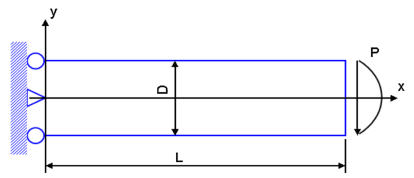
\includegraphics[width=7cm]{images/chapter_elasticity/cantilever_beam}
\end{center}

The exact displacement solution of the problem is given by
\begin{eqnarray}
u_x&=& \frac{Py}{6 \bar{E} I} \left[
(6L-3x)x+(2+\bar{\nu})(y^2-D^2/4)\right] \nn\\
u_y&=&-\frac{P}{\bar{E} I} \left[
3\bar{\nu}y^2(L-x)+(4+5\bar{\nu}) \frac{D^2x}{4}+(3L-x)x^2 \right] \label{eq:chapel:sols1}
\end{eqnarray}
where 
\begin{itemize}
\item plane stress: $\bar{E}=E$, $\bar{\nu}=\nu$
\item plane strain: $\bar{E}=E/(1-\nu^2$, $\bar{\nu}=\nu(1-\nu)$
\end{itemize}
The plane strain condition is studied for volumetric locking, and $I=D^3/12$ is the second
moment of area of the beam. The corresponding stress solutions are

\begin{eqnarray}
\sigma_{xx}(x,y)&=&\frac{P(L-x)y}{I} \nn\\
\sigma_{yy}(x,y)&=&0 \nn\\
\sigma_{xy}(x,y)&=&-\frac{P}{2I}\left( D^2/4 - y^2 \right) \label{eq:chapel:sols2}
\end{eqnarray}

In computation, analytical displacement solution obtained from Equation \eqref{eq:chapel:sols1}
is prescribed along the left boundary, and the parabolic traction 
on the right boundary applies the exact shear stress
solution provided in Equation \eqref{eq:chapel:sols2}. 
In the paper the authors use a coarse discretization of $2\times 10$ elements.

%--------------------------------------
\subsection{Infinite plate with a circular hole}

%--------------------------------------
\subsection{Cook’s membrane}

%--------------------------------------
\subsection{Punching problem}









